\documentclass[a4paper,12pt]{article}
\usepackage{amsmath}
\usepackage{amsfonts}
\usepackage[english]{babel}
\usepackage{fancyhdr}
%\usepackage[prefix]{nomencl}
%\usepackage{makeidx}
\usepackage{cite}
\usepackage{float}
\usepackage{placeins}
\usepackage{graphicx}
\usepackage{epstopdf}
%\usepackage{multicol}
%\usepackage{url}
\usepackage{listings}
\usepackage{pdfpages}
\usepackage[utf8]{inputenc}
\usepackage[hidelinks]{hyperref}
%\usepackage{cleveref}

\usepackage{caption}
%\usepackage{subcaption}
\usepackage{subfig}
\renewcommand{\contentsname}{Innehållsförteckning}
%\hypersetup{linkcolor=blue, colorlinks=true}


%\makenomenclature

\let\oldAuthor\author
\renewcommand{\author}[1]{\newcommand{\myAuthor}{#1}\oldAuthor{#1}}
\renewcommand{\deg}{\ensuremath{^{\circ}}\xspace}

\begin{document}

%---------------------------------------------------------
%Fill in:
% Redaktör
%---------------------------------------------------------

%---------------------------------------------------------
%Fill in:
%1. Redaktör(er)
%3. Organisation/Företag/Institution...
%4. Projektnamn
%5. Projektgrupp, med email eller liknande kontakt uppgift
%6. Granskare av dokument
%7. Datum som graskningen skedde
%8. Godkännare av dokumentet
%9. Datum för godkännande
%---------------------------------------------------------
\title{Project report}
\author{Tobias Nilsson }
\date{} %<-- LEAVE EMPTY! 
\newcommand{\organisation}[0] {\small Institutionen för Fysik \\ Umeå Universitet}
\newcommand{\projektnamn}{\small Upgrade: Electrical Conductivity}
\newcommand{\projektgrupp}{ Tobias Nilsson, \\ toni0042@student.umu.se \\
							 Jesper Vesterberg,\\ jeve0100@student.umu.se}
\newcommand{\granskare}{Jesper Vesterberg}
\newcommand{\granskatdatum}{GRANSKATTDATUM}
\newcommand{\godkannare}{Krister Wiklund}
\newcommand{\godkantdatum}{GODKÄNTDATUM}


\begin{titlepage}
\maketitle 
\thispagestyle{fancy}
\headheight 35pt 
\lhead{\organisation}
\chead{\projektnamn}
\rhead{\small\today}
\cfoot{\projektgrupp}

\begin{center}
Version 1.0
\end{center}

\vspace{80mm}
\begin{center}
  {\large Status:}\\[1.5ex]
  \begin{tabular}{|*{3}{p{40mm}|}}
    \hline
    Reviewed & \granskare & \granskatdatum \\
    \hline
    Approved & \godkannare & \godkantdatum \\
    \hline
  \end{tabular}
\end{center}

\end{titlepage}



\pagestyle{fancy}
\headheight 35pt 
\pagenumbering{roman}
\rhead{\small\today \\ }
\chead{\projektnamn}
\lhead{\organisation \\ }
\lfoot{Projektarbete inom \\teknisk fysik B, 3.0 HP \\ 5FY070}
\cfoot{\thepage}
\rfoot{\projektgrupp}
\begin{center}

\section*{\center Project identity}

\bigskip
\begin{tabular}{|p{35mm}|p{30mm}|p{20mm}|p{45mm}|}
\hline
\textbf{Name} & \textbf{Ansvar} & \textbf{Telephone} & \textbf{e-mail}\\
\hline
Tobias Nilsson & Documents &  & toni0042@student.umu.se\\
\hline
Jesper Vesterberg & Programmer &  & jeve0010@student.umu.se\\
\hline
\end{tabular}

\bigskip
\textbf{Client}: Institutionen för Fysik, Umeå universitet, \\
Linnaeus väg 24,\\
901 87\\
Umeå.

\textbf{Contact}: Krister Wiklund, krister.wiklund@umu.se.
\end{center}
\newpage

\tableofcontents
\newpage
\pagenumbering{arabic}

\section{Introduction}
The purpose of the lab \emph{Electrical conductivity} in the courses \emph{Solid State Physics} is to investigate how the electrical conductivity of different materials behaves in the temperature region $10-300$ $K$. The materials in question are a semi-conductor, InSb, a metal, Pt, and a super conductor, $YBa_2Cu_3O_7$.

The aim of the project was to upgrade the the laboratory equipment, which consisted of; a cryo system, with heat controller; a series of power supplies; a black box with measurement circuits, that converted resistance to voltage; a bench multimeter and an ancient  computer system running on MS-DOS. The upgrades consisted of removing the external power supplies, the black box, exchanging the computer for a newer laptop and the user interface, \emph{Elledn}, was rewritten in Labview.



\section{The set-up}
Equipment consist of:
\begin{itemize}
\item Cryogenic system:
\begin{itemize}
\item Cooling chamber
\item Coarse vacuum pump
\item Turbo molecular pump
\item Cryogenic system(compressor w. cooling system): HC-2, APD Cryogenics Inc.
\end{itemize}
\item Controllers to cryogenic system: 
\begin{itemize}
\item Turbotronic NT10
\item Thermovac TM20
\item Scientific Instruments Inc. 9620-1 Silicon Diode
\end{itemize} 
\item Bench Multimeter: Keithley 2001 Multimeter
\item Computer with Labview.
\end{itemize}

The materials are placed in the cooling chamber and the two vacuum pumps reduces the pressure to below $10^{-5}$ Pascal. This reduces the amount of heat that needs to be removed to change the chambers temperature. Remember the ideal gas law $PV=NkT$. The actual cooling process is a closed helium-gas cycle that follows the Gifford-McMahon principle.

The samples are continuously cooled by the equipment to $\approx 10$ $K$ if no additional heat is added. Thus to change the temperature additional heat is added to the system by an external heater. This heater is controlled by the \emph{Scientific Instruments Inc. 9620-1 Silicon Diode}. Which in turn can be controlled by a computer through an GPIB-interface and its front panel. 

The controller determines the heating with the aid of the PID equation, consisting of a \textbf{P}roportional, an \textbf{I}ntegral and a \textbf{D}ifferential term. To improve the performance and responsiveness of the cryogenic equipment in various temperature ranges, the coefficients for these terms can be changed by the user. For more information see equation \eqref{eq:PID} and the \emph{Scientific Instruments Inc. 9620-1 Silicon Diode manual}.

To determine the resistivity of the samples, each sample is connected to a 4 sense wire system. These sense wires are connected to a Keithley 2001 Multimeter through a switching card at the back of the multimeter. The multimeter is also equipped with a GPIB-interface, enabling computer controlled measurements. 

The connections from the samples and an additional temperature diode, goes first a through a round 19 pin contact to an 25 pin d-sub connector. See table \ref{tab:PinNumbers} for pin layout on the cables.

\begin{table}[H]
	
  \caption{\emph{Pin layout for connection cables between cooling chamber and multimeter. Ports 19-24 on the 25-pin Dsub connector are  unused.}} 
  
  \begin{tabular}{c|c|c c c}
  \label{tab:PinNumbers}
  25-pin D-sub & round 19-pin connector & Function & & \\
  \hline
  1  & A & Superconductor    & Current & + \\
  2  & B & ''                & ''      & - \\
  3  & C & ''                & Voltage & + \\
  4  & D & ''                & ''      & - \\
  5  & E & Conductor, Pt-100            & Current & + \\
  6  & F & ''                & ''      & - \\
  7  & G & ''                & Voltage & + \\
  8  & H & ''                & ''      & - \\
  9  & J & Semi-conductor, InSb-plate        & Current & + \\
  10 & K & ''                & ''      & - \\
  11 & L & ''                & Voltage & + \\
  12 & M & ''                & ''      & - \\
  13 & N & Temperature diode & Current & + \\
  14 & P & ''                & ''      & - \\
  15 & R & ''                & Voltage & + \\
  16 & S & ''                & ''      & - \\   
  17 & T & free              &         &  \\
  18 & U & free              &         &  \\
  25 & V & Shield            &         &  \\ 
  \end{tabular}
  
\end{table} 




The samples are connected to the Keithley Multimeter through a custom scanning card. This card enables the use of the built-in switching capabilities and it has two rows of pins, a red (positive) and a black (negative). When using this home made card for 4-wire measurements it can be important to know that the first five pins (pins 1-5) are used for the potential wires and that the  last five (pins 6-10) are used for the current wires.

The first potential pins are grouped with the first current pins, e.g. pins 1 and 6 are connected two sample 1 and pins 2 and 7 are connected to sample 2 and so on. See Table \ref{tab:ScanCard} for details about how the samples currently are connected to the scanning card.
 
 
 \begin{table}[H]
	\center
	
	\caption{\emph{Pin layout for the Scan card, inside the Keithley Multimeter.}} 
	\begin{tabular}{l|l|l}
	\label{tab:ScanCard}
		\#  & +(Red) & -(Black) \\
		\hline
		1  & Superconductor, Potential +	& Superconductor, Potential - \\
		2  & Semi-conductor, Potential +		& Semi-conductor, Potential - \\
		3  & Conductor, Potential +			& Conductor, Potential - \\
		4  & 	N/A	& N/A \\
		5  & 	N/A	& N/A \\
		6  & Superconductor, Current +		& Superconductor, Current - \\
		7  & Semi-conductor, Current +		& Semi-conductor, Current - \\
		8  & Conductor, Current +			& Conductor, Current - \\
		9  & 	N/A	& N/A \\
		10 & 	N/A	& N/A \\
	\end{tabular}
	
\end{table}

\section{Software}

This section describes shortly how the software works. For a guide on how to operate the software see the laboratory instructions for electrical conductivity. 

The software, ResSolidLabV1 (see figure \ref{fig:UI} for a snap shot), is written in Labview and its user interface has a reduced control of the measurement system. For simplicity it can only change the temperature and initiate measurements. All other changes in the measurement system, has to be done outside the user interface. Such as changing the different coefficients in the PID equation that controls the heating element. 


\begin{figure}[H]
\center
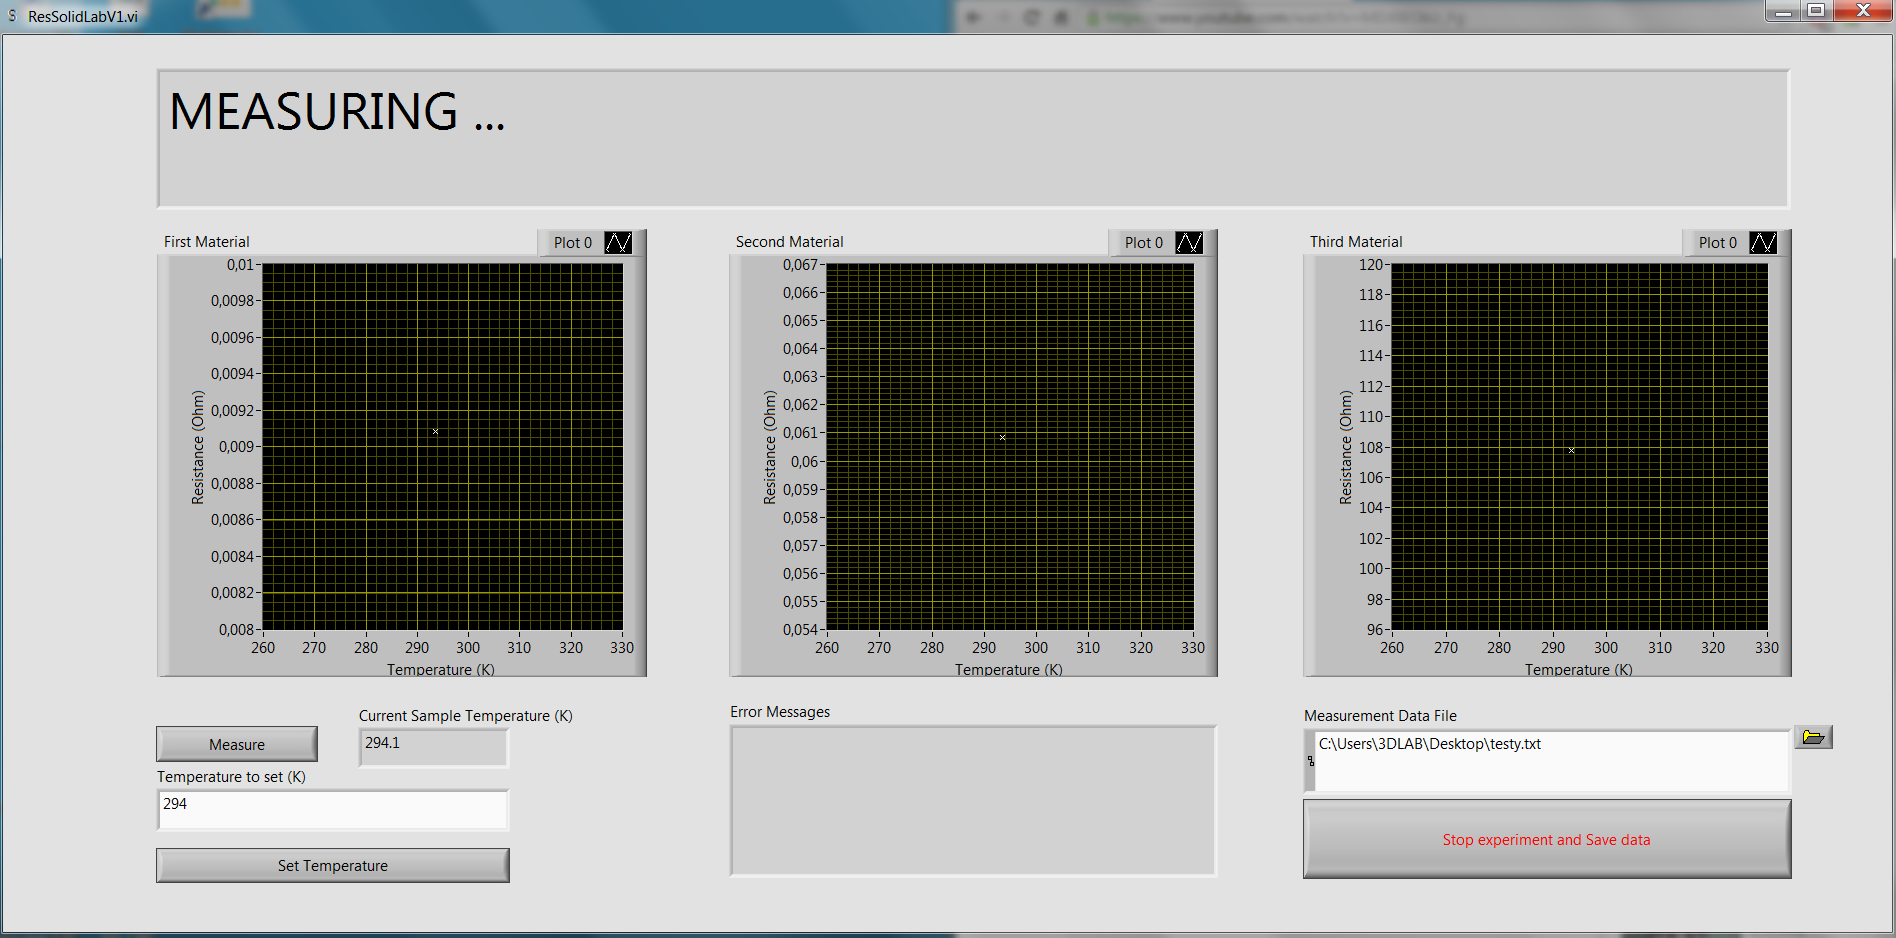
\includegraphics[width=1\textwidth]{ResSolidLabV1UI.PNG}
\caption{\emph{Snapshot of the ResSolidLabV1's user interface.}}
\label{fig:UI}
\end{figure}

However the bench-multimeter's settings are made automatically by ResSolidLabV1, these settings are about how the measurements are performed and the change these settings, the parts of the program needs to be rewritten.

JESPER! FYLL I HÄR VILKA SAKER SOM ÄR "HÅRDKODADE" I PROGRAMMET OCH HUR MAN ÄNDRAR PÅ DEM!!!!!!!!!!!!!!

The  bench-multimeter can not truly measure zero resistance even with the 4-wire setup and the measured values are often negative. The solution implemented in the software is to chose the maximum value between the measured resistance and zero. This introduces a potential problem. Switching place of either the current or resistance cables will change the sign of the measure resistance.


\section{Hardware}

\subsection{Keithley 2001 Multimeter}

VILKA KOMMANDON FINNS DET, VILKA PORTAR PÅ DET HEMMA GJORDA KORTET HÖR IHOP.

\subsubsection{GPIB-Commands and related: Multimeter}

\paragraph{Current GPIB-address}

\paragraph{Change GPIB-address}

\paragraph{Set up 4-wire}

\paragraph{Set up number of averages etc. etc.}

\paragraph{Switch channels}

\paragraph{Do measurement}


\subsection{Heater control: \\ Scientific Instruments Inc. 9620-1 Silicon Diode}
The Scientific Instruments Inc. 9620-1 Silicon Diode is the controller that sets the heat, as previous stated it governed by the PID equation, which typically looks like this:

\begin{equation}
u(t)= K_pe(t) + K_i\int_0^t \! e(\tau)\mathrm{d}\tau + K_d\frac{\mathrm{d}e(t)}{\mathrm{d}t}.
\label{eq:PID}
\end{equation}

\noindent Here $u(t)$ is the power of the heater and $e(t)$ is the error in temperature compared to the wanted temperature. The coefficients $K_p$, $K_i$ and $K_d$ are constant and larger than zero. They can be set by the user, but since the system is working good enough there is no reason to tamper with them. 

\subsubsection{GPIB-Commands and related: Heater}

\paragraph{Current GPIB-address}

\paragraph{Change GPIB-address}

\paragraph{Temperature}

\paragraph{Set Temperature}





%\begin{appendix}


%Here you can put additional data of importance Labview or Matlab codes,
%additional equations and derivations etc.
%Do not add long tables of raw data. 
%
%For programming code like Matlab you need to use a font where 
%all letters are equally wide. Use the verbatim environment.
%
%\begin{verbatim}
%	Paste code here! 
%\end{verbatim}

%\section{Appendix section 2} 

%\end{appendix}

\end{document}